
\documentclass[a4paper,12pt]{article}
\usepackage{epstopdf}
\usepackage[utf8]{inputenc}
\usepackage[swedish]{babel}
\usepackage{enumerate}
\usepackage{mathtools}
\usepackage{hyperref}
\usepackage{float}
\usepackage[pdftex]{graphicx}   
\usepackage{multirow}
\usepackage{listings}
\lstset{
    language=R,
    basicstyle=\ttfamily
}

\title{TDDE01 -- Machine Learning \\
       Individual Lab Report 3}
\author{Martin Estgren \texttt{<mares480>}}
      
\begin{document}
 \pagenumbering{arabic}
    \maketitle % Generate.
\section{Assignment 1}

This assignment involves creating an implementation of the \textit{linear discriminant analysis} (LDA) with \textit{maximum likelihood estimation} (MLE) as \textit{discrimination function}. The LDA function will then be used to classify the \textit{sex} of Chicago crabs using the \textit{carapace length} and the \textit{rear width} from the data set given for the assignment.

The first step involves visual inspection of the data set to determine if a \textit{linear discrimination function} would be a good fit for the data set. The result of the \textit{response variable} \textit{sex} is ploted as the color of each point with the predictors \textit{carapace length} and \textit{rear width} as X and Y dimensions.

\begin{figure}[H]
\centering
\begin{minipage}[]{0.5\textwidth}
  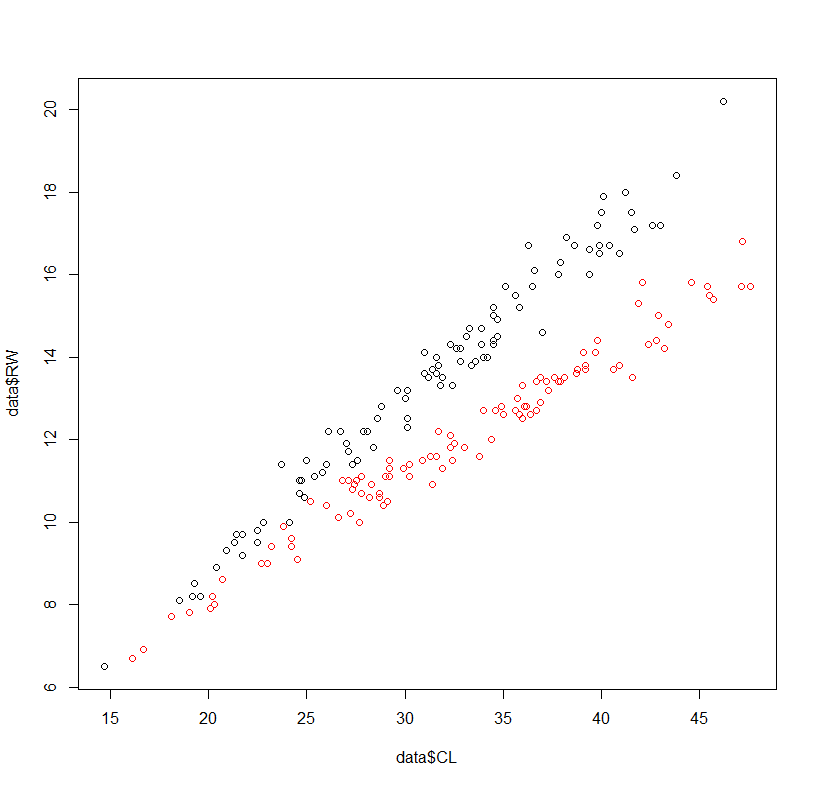
\includegraphics[width=\textwidth]{figures/raw_plot.png}  
  \caption{Raw plot of the data set.\label{fig:raw_plot}}
 \end{minipage}
\end{figure}
Visual inspection of the data set indicates that a linear classification model would be suitable.

In order to implement the LDA function we start by implementing the MLA and return the weights for each classification category. 

\begin{equation}
    w_{1i} = -\frac{1}{2}\mathbf{\mu}^{T}_i\Sigma^{-1}\mathbf{\mu}_i+log \pi_i
\end{equation}
where $i \in \{CL,RW\}$

\begin{equation}
    b_{1i} = \Sigma^{-1}\mathbf{\mu}_i
\end{equation}
The classification function can be derived form these variables by combining them into:
\begin{equation}
  d_i(x) = X^T \Sigma^{-1}\mathbf{\mu}_i -\frac{1}{2}\mathbf{\mu}^{T}_i\Sigma^{-1}\mathbf{\mu}_i+log \pi_i
\end{equation}
In our case we have two categories for the classifier: $\{Male,Female\}$ which means that we need to combine the two different $d_i(x)$ functions with $d(x) = d_{Male}(x) - d_{Female}(x)$. We are in addition to classifying the data points interested in drawing the LDA line in the plot. In order to do this the intercept and slope of the LDA function is calculated from the $d(x)$ in the following way:

\begin{equation}
  intercept = \frac{-b_1}{w_{1RW}}
\end{equation}
\begin{equation}
  slope = \frac{-w_{1CL}}{w_{1RW}}
\end{equation}
The resulting plot can be seen below
\begin{figure}[H]
\centering
\begin{minipage}[]{0.5\textwidth}
  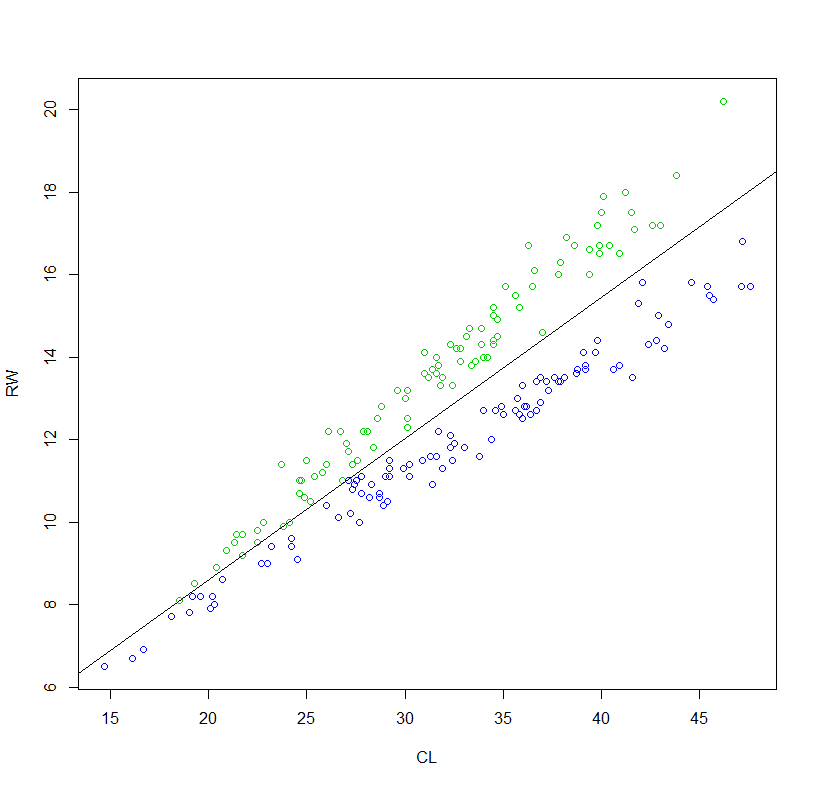
\includegraphics[width=\textwidth]{figures/lda_plot.png}  
  \caption{Plot of the raw data classified with LDA.\label{fig:lda_plot}}
 \end{minipage}
\end{figure}
The misclassification rate is 0 meaning the result is a close to perfect classification. 

As observed in above, the LDA managed to perform a perfect classification. The next task involves using the built in \textit{logistic regression} classifier and examine its performance on the same data set.

Once again we extract the coefficients from the discriminant model and plot both the predicted result together with the \textit{discrimination bound}.

\begin{figure}[H]
\centering
\begin{minipage}[]{0.5\textwidth}
  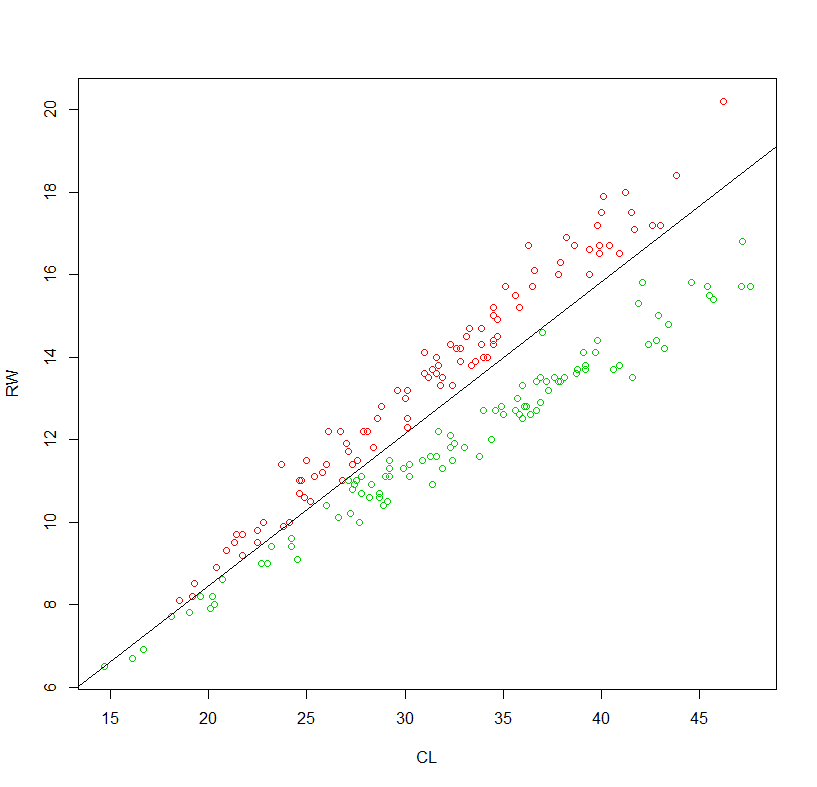
\includegraphics[width=\textwidth]{figures/logit_plot.png}  
  \caption{Plot of the raw data classified with logistic regression.\label{fig:logit_plot}}
 \end{minipage}
\end{figure}
The \textit{logistic regression} also managed a similar classification of the given data set with.

\section{Assignment 2}

In this assignment we are tasked with finding a classification model to find potential good customers who can manage their loans in a "good" way. To achieve this we use a data set with observations about how previous customers has manged their loans given a set of predictors. 

We start by splitting the observations into 50,25,25 percent parts and try fitting a decision tree model based on \textit{deviance} and \textit{gini index}. Below are the confusion matrices and misclassification rates for the testing and training observations.

Below the two different types of description trees can be observed followed by the confusion matrices and miss classification rate.
\begin{figure}[H]
\centering
\begin{minipage}[]{0.49\textwidth}
  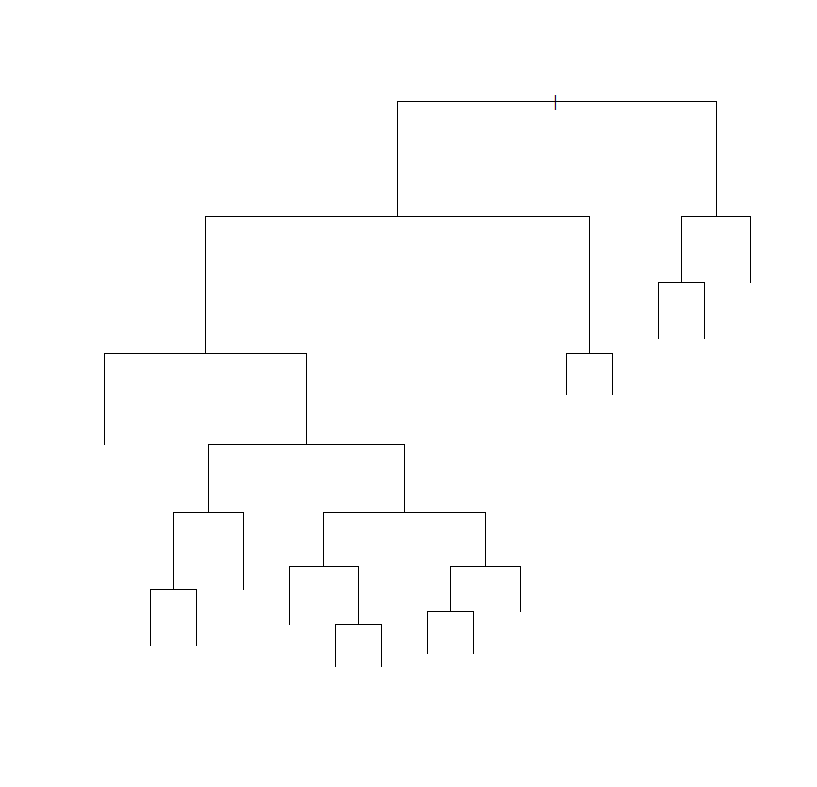
\includegraphics[width=\textwidth]{figures/deviance_table.png}  
 \end{minipage}
 \begin{minipage}[]{0.49\textwidth}
  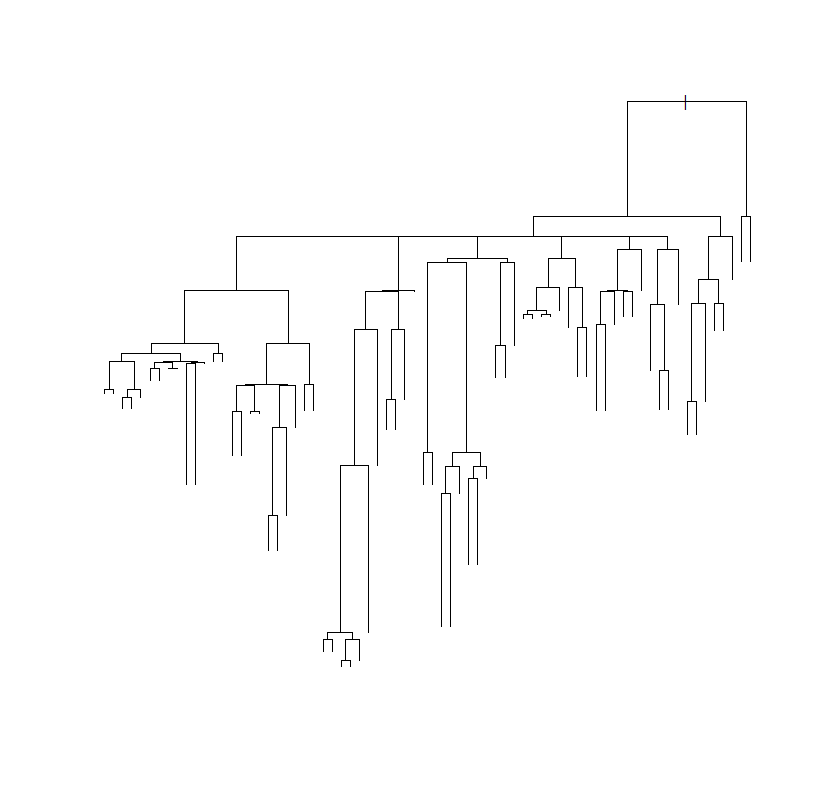
\includegraphics[width=\textwidth]{figures/gini_table.png}  
 \end{minipage}
\end{figure}
The \textit{deviance} metric created a much less complex tree compared to the \textit{gini index}. This is mirrored in the misclassification ate where the \textit{deviance} creates the best result.

\begin{minipage}[]{0.49\textwidth}
 \begin{verbatim}
deviance model fitness
       predicted
       bad good
  bad   29   17
  good  45  159
misclassification rate: 0.248
\end{verbatim}
 \end{minipage}
 \begin{minipage}[]{0.49\textwidth}
\begin{verbatim}
gini model fitness
       predicted
       bad good
  bad   24   26
  good  50  150
misclassification rate: 0.304
\end{verbatim}
 \end{minipage}

In order to determine the best max tree depth of the \textit{deviance} model we iterates through all depths between 2 and 15.
\begin{figure}[H]
\centering
\begin{minipage}[]{0.5\textwidth}
  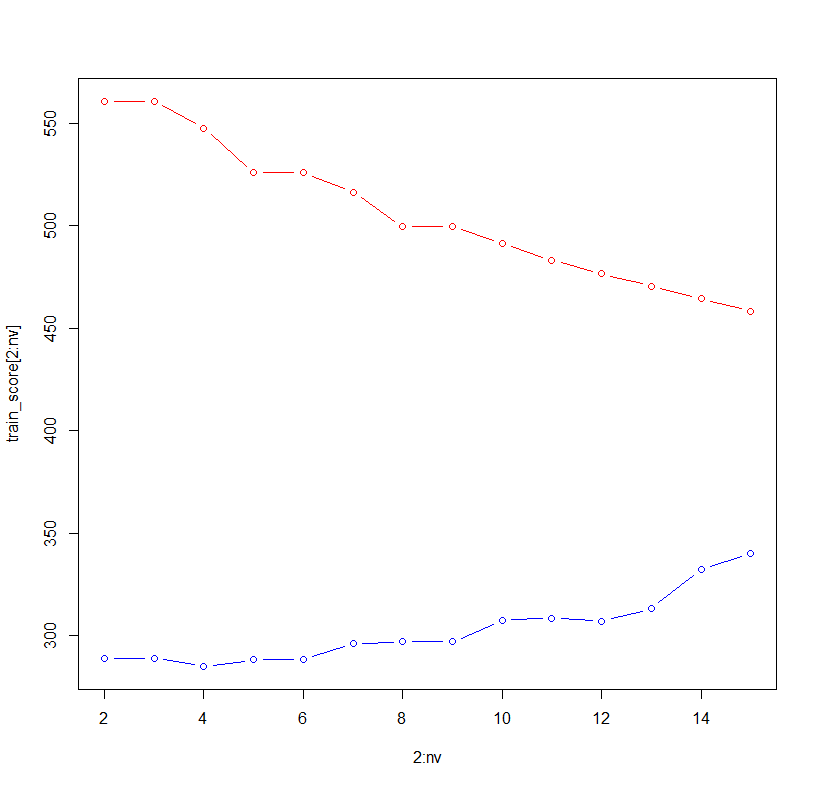
\includegraphics[width=\textwidth]{figures/tree_depth.png}  
  \caption{deviance for different max tree depths.\label{fig:logit_plot}}
 \end{minipage}
\end{figure}
The \textit{red} line indicates deviance of the training data and the \textit{blue} line, the validation data. Tree depth of 4 results in the least deviance for the training data.

\begin{verbatim}
optimal depth deviance fitness
       predicted
       bad good
  bad   20   59
  good   9  162
misclassification rate: 0.272
\end{verbatim}

\begin{figure}[H]
\centering
\begin{minipage}[]{0.5\textwidth}
  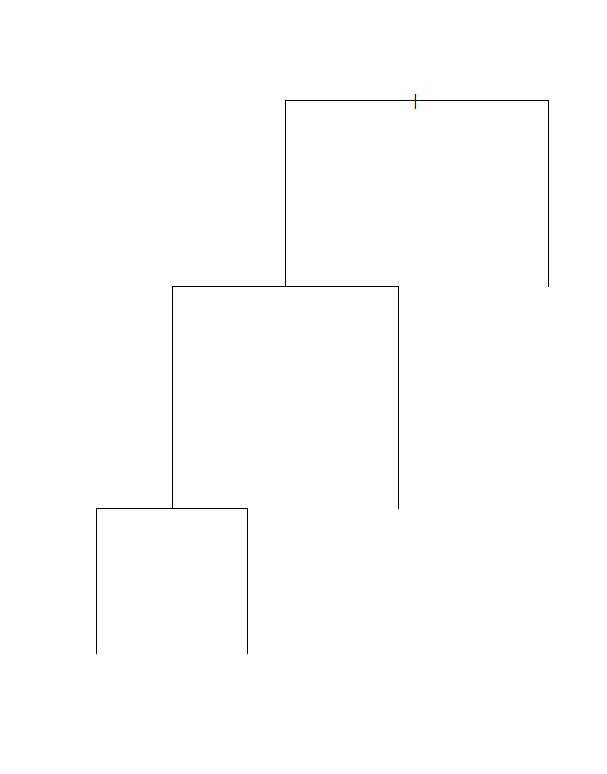
\includegraphics[width=\textwidth]{figures/best_subtree.png}  
  \caption{Optimal tree model. \label{fig:best_subtree}}
 \end{minipage}
\end{figure}

The following confusion matrix represents the same data set used on a \textit{naive bayesian} model instead of a decision tree.

\begin{verbatim}
model fitness of the training set
      predicted
      bad good
bad   95   98
good  52  255
misclassification rate: 0.3
\end{verbatim}
\begin{verbatim}
model fitness of the testing set 
      predicted
      bad good
bad   52   53
good  22  123
misclassification rate: 0.3
\end{verbatim}
We can observe about the same misclassification ratio as the decision tree model. The training data predictions have about the same level of misclassification as the testing set but with a higher level of true positives.

We now apply a \textit{loss matrix} to the predictions of the model and compare the result to the result above. The loss matrix looks the following:

\begin{equation}
  \begin{bmatrix}
  0 & 1\\ 
  10 & 0
  \end{bmatrix}
\end{equation}

\begin{verbatim}
model fitness of the training set
      predicted
truth bad good
bad   27   17
good  120  336
misclassification rate: 0.274

model fitness of the testing set
      predicted
truth bad good
bad  18  10
good 56  166
misclassification rate:0.264
\end{verbatim}
The result indicates a improvement in performance of about 2-3 percent.

\section{Appendix: A - Code assignment 1}

\lstinputlisting[caption=Code for assignment 1,
    label={code/assignment1.r},
    breaklines=true]
    {code/assignment1.r}

\section{Appendix: B - Code assignment 2}

\lstinputlisting[caption=Code for assignment2 ,
    label={code/assignment2.r},
    breaklines=true]
    {code/assignment2.r}

\end{document}
